\subsection{REQUESTPROXY (96)}

The REQUESTPROXY message is sent by the parties of the file transfer to verious
nodes in the following mannger: The encrypted part of the OFFER message contains
a list of "part data" structures. Each part data represents a part of the
transfered file. Each such part will be sent by the offerer to a different node,
randomly chosen from its list of neighbors before initiating an offer. If he
does not have enough neighbors, then more addresses should be requested from a
DNL node using PULL. Before making the offer, the offerer has to request the
randomly chosen nodes to have the role of proxies in the transfer, using the
REQUESTPROXY message. A node may or may not accept such a request. When
accepting, we say that the node becomes a "drop point" in this transfer. When
the transfer begins, the offerer will start uploading a part of the file to each
drop point. The party which requested the respective file will know where to get
the parts - the addresses are recorded in the part data structures.

This message type will also be utilized by the file requester, as he will not
retrieve the parts directly from the drop points, but will ask other nodes to
do this on his behalf. These nodes are called "lift proxies".

The message content only has one field, the size of the part to be handled by
the proxy. The status code specified whether or not the node accepts to have the
role of lift proxy or drop point. The acceptance criteria are dependent on
implementation or configuration.

\begin{figure}[H]
    \centering
    \scalebox{.33}{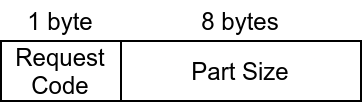
\includegraphics{figures/requestproxy}}
\end{figure}

\subsection{CANCELPROXYREQUEST (97)}

A proxy request may be canceled by one of the parties. This type of message is
implementation defined and may not be implemented at all if not needed.

\subsection{INITUPLOAD (98)}

INITUPLOAD is used to initialize a part upload between nodes. The upload
procedure initialized by this message is performed:
\begin{itemize}
    \item From file offerer to drop point.
    \item From lift proxy to file requester.
\end{itemize}

The OfferId is used to identify the transfer and the file. The drop point will
know how large is the part based on the REQUESTPROXY message received earlier,
matched against the address of the message sender.

\begin{figure}[H]
    \centering
    \scalebox{.33}{
\includegraphics{figures/initupload}}
\end{figure}

\subsection{UPLOAD (99)}

The start of the part upload sequence by a node has to be preceded by an
outgoing INITUPLOAD message or an incoming INITDOWNLOAD message. The part is
transfered in chunks, using multiple UPLOAD messages. The transfer is
identified by the part receiver by matching the sender address of the
INITUPLOAD and UPLOAD messages. The file chunks may be sent out of order, and
thus the message contains the chunk offset in the current part. The proxies
involved in the transfer won't need to know the offset of the part in the file.
The part is encrypted by the file offerer before uploading it to the drop
point, using the transfer key recorded in the OFFER message. In this way, only
the the two main parties involved in the transfer are able to view the file
without fearing that a third party may intercept the transfer and read the file
content. A node involved in the transfer does not have to wait for the whole
part before sending the received chunks to the next hop.

\begin{figure}[H]
    \centering
    \scalebox{.33}{
\includegraphics{figures/upload}}
\end{figure}

\subsection{FETCH (100)}

FETCH is the message send by the file requester to a lift proxy to ask it to
fetch a file part from a drop point. The "Address" field specifies the address
of the drop point.

\begin{figure}[H]
    \centering
    \scalebox{.33}{
\includegraphics{figures/fetch}}
\end{figure}

\subsection{INITDOWNLOAD (101)}

INITDOWNLOAD is sent by a lift proxy to a drop point, to inform the drop point
node to start uploading the stored file part associated with the given OfferId
to the lift proxy.

\begin{figure}[H]
    \centering
    \scalebox{.33}{
\includegraphics{figures/initdownload}}
\end{figure}
